%!TEX root = ../paper.tex

\begin{figure}
	\centering
	%!TEX root = ../paper.tex
%Ferdosi Sets 1
\begin{subfigure}{0.23\textwidth}
	\centering
	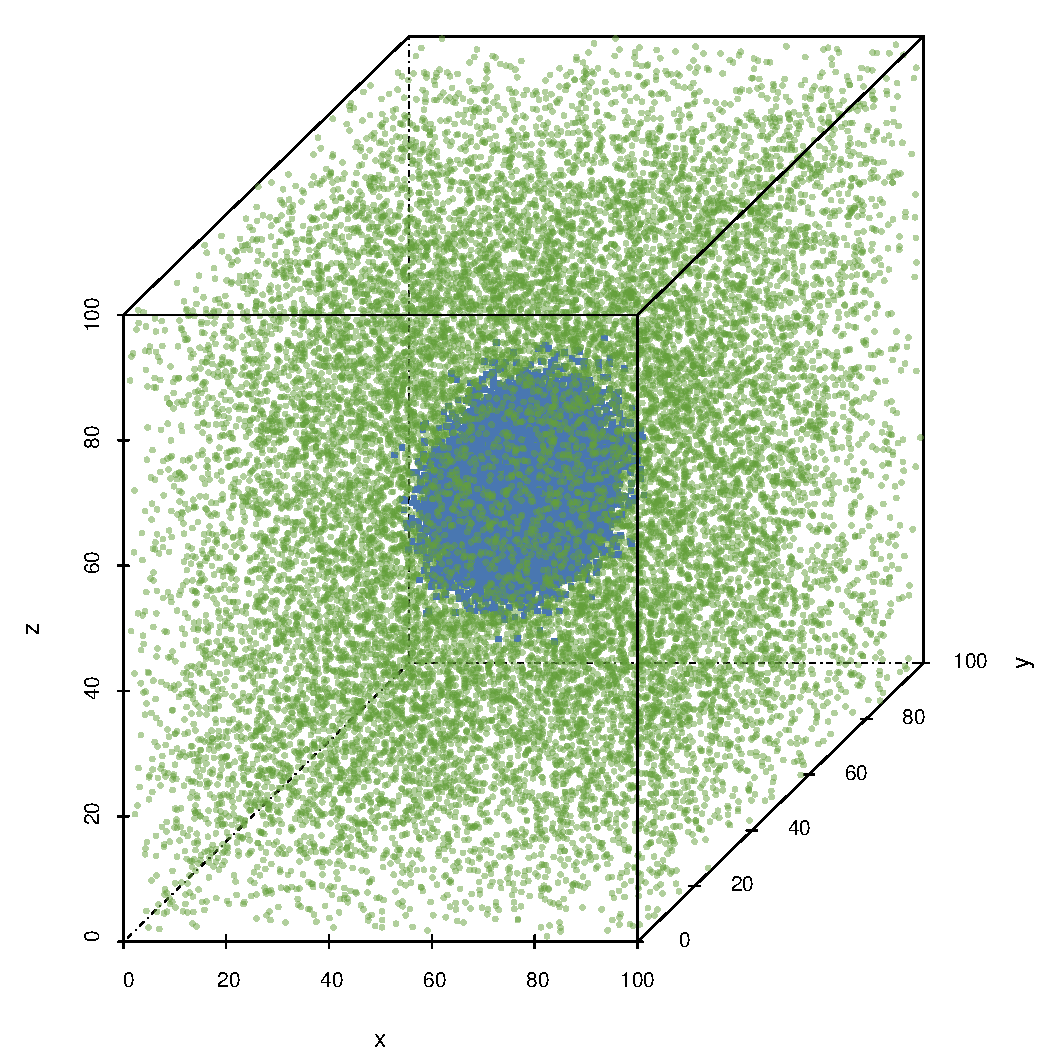
\includegraphics[width=\textwidth]{experiment/img/datasetplot_ferdosi_1_60000}
	\caption{Set \ferdosiOne}
	\label{fig:3:simulated:datasets:ferdosi1}
\end{subfigure}
% Baakman 1	
\begin{subfigure}{0.23\textwidth}
	\centering
	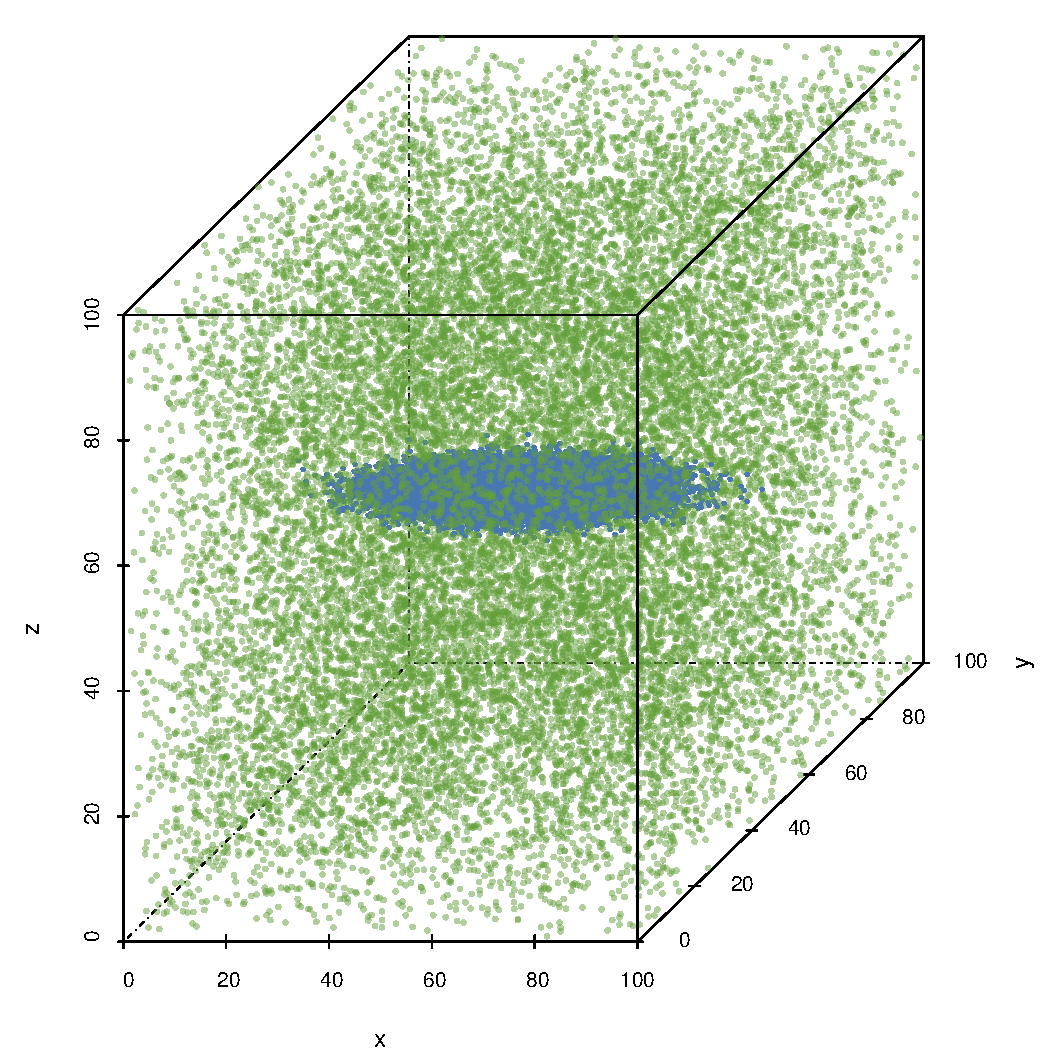
\includegraphics[width=\textwidth]{experiment/img/datasetplot_baakman_1_60000}
	\caption{Set \baakmanOne}
	\label{fig:3:simulated:datasets:baakman1}
\end{subfigure}
% Baakman 4
\begin{subfigure}{0.23\textwidth}
	\centering
	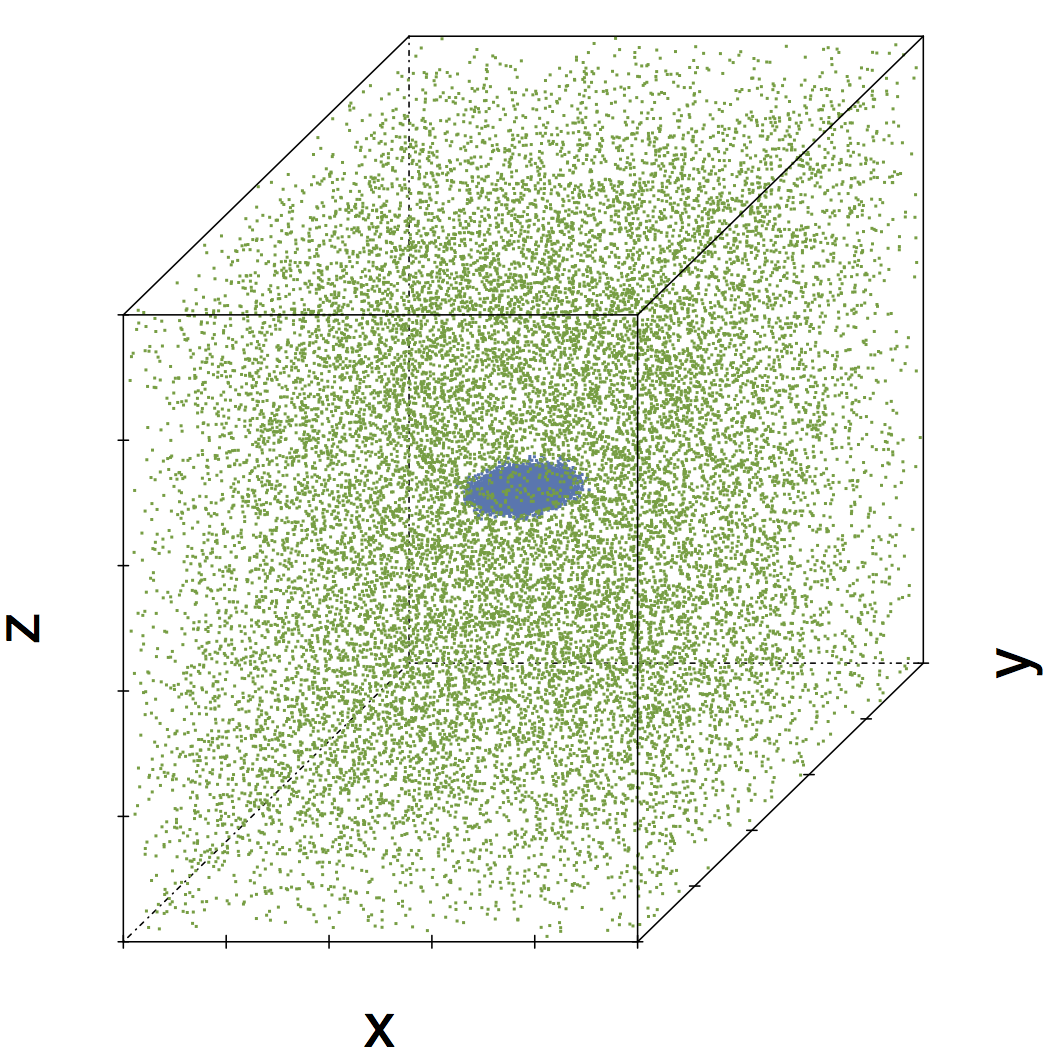
\includegraphics[width=\textwidth]{experiment/img/datasetplot_baakman_4_60000}
	\caption{Set \baakmanFour}
	\label{fig:3:simulated:datasets:baakman4}
\end{subfigure}	
% Baakman 5
\begin{subfigure}{0.23\textwidth}
	\centering
	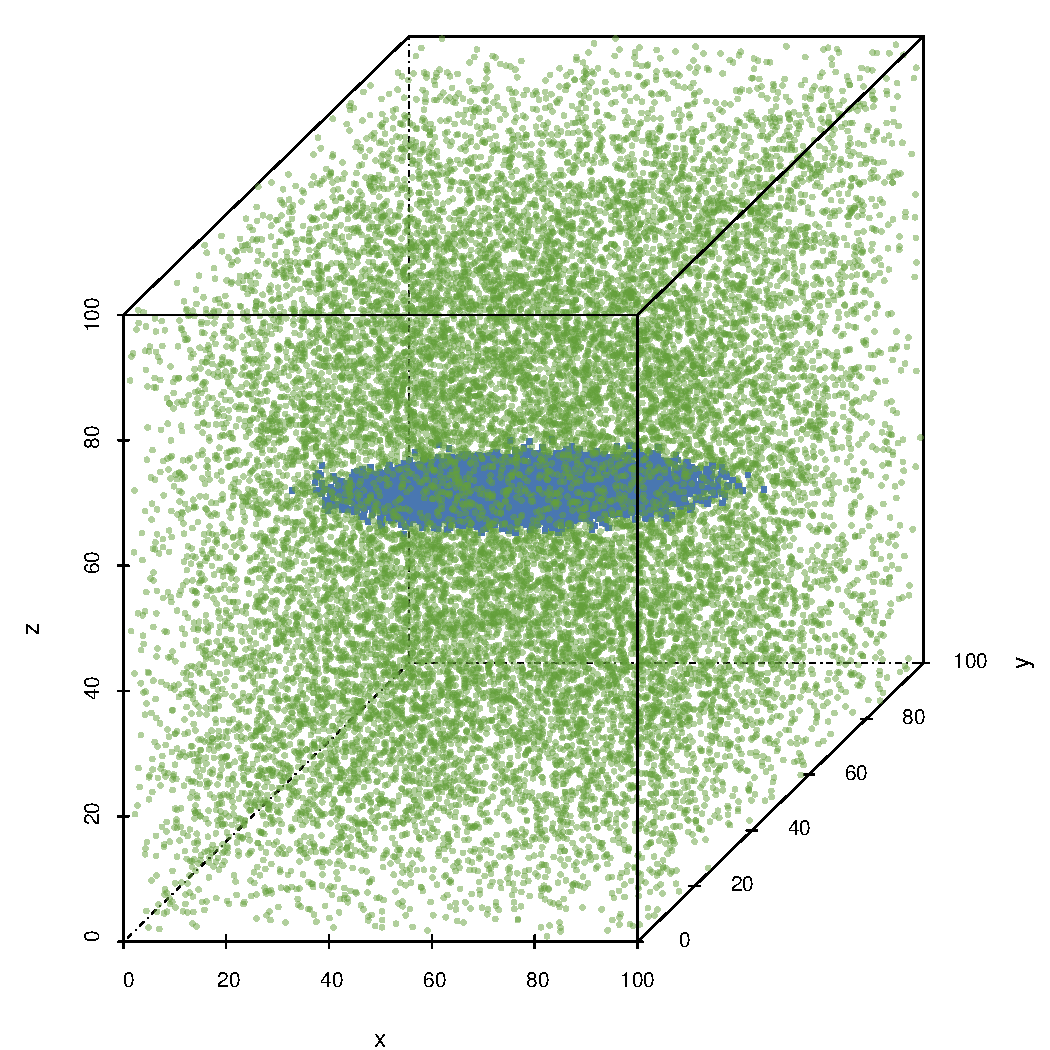
\includegraphics[width=\textwidth]{experiment/img/datasetplot_baakman_5_60000}
	\caption{Set \baakmanFive}
	\label{fig:3:simulated:datasets:baakman5}
\end{subfigure}	
	\caption{Plots of the density estimated by \mbe versus the density estimated by \sambe of dataset %
		\subref{fig:discussion:singlesphere:mbevssambe:ferdosi1} \ferdosiOne, %
		\subref{fig:discussion:singlesphere:mbevssambe:baakman1} \baakmanOne, %
		\subref{fig:discussion:singlesphere:mbevssambe:baakman4} \baakmanFour, and %
		\subref{fig:discussion:singlesphere:mbevssambe:baakman5} \baakmanFive, %
	The black line represents the function $f(x) = x$.}
	\label{fig:discussion:singleSphere:mbevssambe}
\end{figure}

%General Discussion
	%Small difference between two estimators
		% Confirm with plots
		The most striking observation of \cref{s:results:singleGaussian} is the small difference between the densities approximated by the two estimators. To investigate what caused these differences we first investigated if the differences in \mse were not caused by a select group of points, to that end we plotted the density estimated by \sambe as a function of the density estimated by \mbe, see \cref{fig:discussion:singleSphere:mbevssambe}. These plots do not indicate a specific group of points that causes the difference in \MSE between the two estimators within datasets.
		
		% Investigate the points with the largest differences
		Investigating the points that lie farthest from the line $x = x$ in the plots in \cref{fig:discussion:singleSphere:mbevssambe} we find that in the datasets with a single Gaussian they all lie near the mean of the Gaussian distribution. Furthermore the density of these points are both over and underestimated by the shape-adaptive estimator, if the first is the case generally fewer points have contributed to the \mbe density than to the \sambe density. If the shape-adaptive estimator underestimates densities it generally uses far less points to base its approximation on than the symmetric estimator uses for that same point. This suggest that some of the kernels near the mean of the Gaussian our to big, allowing a contribution to some points that they should not contribute to, and conversely that some are too small. 

		% Investiage the kernels.
		Reviewing the shape of the kernels used by the shape-adaptive estimator we find some differences between the datasets. 
			% Ferdosi 1
			In dataset \ferdosiOne, as expected due to the spherical Gaussian, the three eigenvalues of the kernels hardly differ, indicating that the kernels are near spherical. 
			% Baakman 1
			The elongated version of this dataset, there are a couple of points with ellipsoidal kernels, as indicated by the eigenvalues of their covariance matrices. Since all these points are positioned in corners of the dataset we contribute the shape of these kernels to their position, instead of to any influence from the Gaussian distribution. 
			% Baakman 4
			
		% Baakman 4
			% EigenValues
			% Eigenvalues indicate about 100  points have kernels with an decideldly non-spherical shape. No pattern in location. 

		% Baakman 5 
			% EigenValues
			% Eigenvalues indicate some points have kernels with a more or less non-spherical shape. No pattern in location. 		

% Dataset Specific Observations?